%\documentclass{article}
%\usepackage{amssymb}
%\usepackage{wasysym}
%\usepackage{graphicx}
%\usepackage{bm}
%\usepackage{psfig}
%\newcommand{\bc}{\begin{center}}
%\newcommand{\ec}{\end{center}}
%\newcommand{\be}{\begin{equation}}
%\newcommand{\ee}{\end{equation}}
%\newcommand{\bea}[1]{\begin{eqnarray}\label{#1}}
%\newcommand{\eea}{\end{eqnarray}}
%\newcommand{\bua}{\begin{eqnarray*}}
%\newcommand{\eua}{\end{eqnarray*}}
%\newcommand{\infint}{\int_{-\infty}^{\infty}}
%\newcommand{\dd}[2]{{{d#1}\over{d#2}}}
%\newcommand{\ddt}[1]{\dd{#1}{t}}
%\newcommand{\dddt}[1]{\dd{^2#1}{t^2}}
%\newcommand{\aver}[1]{\langle{#1}\rangle}
%\def\cl#1{{\cal #1}}               % for caligrafic letters
%\def\labs{\mid\!}
%\def\rabs{\!\mid}
%\begin{document}
%\setcounter{section}{11}
\newcounter{count}
\setcounter{count}{\value{enumi}}
\chapter{Photometry}

The brightness of stars has, along with their locations, been studied
by astronomers since ancient times. Prior to the 1860's observers
necessarily estimated brightness using their eyes expressing the
result in the {\it magnitude system} that Ptolemy introduced in the
second century. 

\section{A short history}

Modern instruments show that early measurements such as those made by
Ptolemy and Tycho Brahe (who were both more interested in the position
of objects) have an internal precision of about $0.5^{\rm m}$. Even a
very skilled observer can do little better; al Sufi in the ninth
century spent great effort on this problem and achieved a precision of
some $0.4^{\rm m}$. With a telescope several observers, such as the Herschels, were able to
produce results of $0.1-0.3^{\rm m}$ by using comparisons with known
{\it sequences} of standard brightness stars. 

Francois Arago suggested an optical/mechanical system by which adjusts
the brightness of a comparison star until it matches the unknown star
or dims the telescopic brightness of a star until it disappears. These
systems are called  {\it visual photometers}. Between 1879 and 1902
Harvard visual photometrists had measured the magnitudes of some
$47\,000$ stars with a precision of about $0.08^{\rm m}$ and an
accuracy of better than $0.25^{\rm m}$. At this time in history (1900)
the Pogson normal scale
\[
\Delta m=-2.5\log({b_1/b_2})
\]
where $b_1$ and $b_2$ are the brightness of objectes $1$ and $2$ was
standard amongst all astronomers. 

\begin{enumerate}
\item The faintest stars visible to the naked eye, from the definition
  of the scale, are magnitude six. For point sources the brightness is
  increased by the use of a telescope by a factor $G$, called the
  light grasp. If the dark adapted human eye has a diameter of 7~mm,
  show that 
\[
G\approx 2\times10^4 d^2
\]
where $d$ is the telscope diameter in meters. Show further that the
limiting magnitude through a visually used telescope, $m_{\rm L}$ is 
\[
m_{\rm L}=16.8+5\log d.
\]
\setcounter{count}{\value{enumi}} 
\end{enumerate}

In the same period photography progressed and astronomers were able to
record the light of stars too faint to be seen by eye in any
telscope. An international collaboration, the {\it Carte du Ciel}
project, was started with the goal of photographing the entire sky and
measuring the brightness of every star below $11.0^{\rm m}$. However,
photographic plates do not measure light linearly and it took several
years, until 1900--1910, before a reliable {\it photographic
  magnitude} system was established. The introduction of physical
photometers in the period 1910--1920 to objectively measure images on
photographic plates eventually led to magnitudes being measured with
uncertainties in the range $0.015-0.03^{\rm m}$.

Experiments with photoelectric work began in the early part of the
20th century and in the 1930's with the introduction of vacuum-tube
amplifiers detection limits on a 0.5~m telescope improved from
$11.0^{\rm m}$ to $13.0^{\rm m}$. Photomultiplier tubes, introduced
during World War {\sc ii}, improved the situation greatly and quickly
became the instrument of choice for measuring brightness, with
uncertainties of $0.005^{\rm m}$ in relative brightness. During the
1950 period to 1980 the RCA~1P21 photomultipliers were used by Harold
Johnson to define the UBV system, which later was extended by the use
of red sensitive photomultipliers into the infrared. 

At present CCDs and other modern solid-state detectors have mostly superseded
photomulitipliers. In the optical CCDs have superior efficiency,
better stability, and a large multiplex advantage.

From space, for example the Kepler mission for detecting occultations
by extrasolar planets, achieves uncertainties below $10~\mu{\rm m}$
over time scales of several weeks.

\section{The response function}

A photometric device is sensitive over a restricted range of
wavelengths called a bandpass. There are three types of bandpass
photometry in astronomy.

\subsection{Types of photometry}

\paragraph{Single-band photometry} For applications such as finding
planets via occultations where one is only interested in measuring the
fraction of light from the star blocked by a planet one needs only a
single band. In this case one would generally want to construct a
sequence of observations into a time series, {\it i.e.} a tabulation
of brightness as a function of time, choosing a wide band to maximize
signal and minimize the required exposure time and telescope size. An
example of this is the Super Wasp telescope arrays placed on La Palma
and in South Africa.
\paragraph{Broadband multi-color photometry} Broadband multi-color
photometry measures a very low resolution spectrum by sampling the
brightness in several different bands. Broad band in this sense means
that the spectroscopic resolving power $R={\lambda_{\rm c}/\Delta
\lambda} < 10-15$. These system attempt to choose bands that admit the
maximum amount of light while still providing astrophysical
information. The most typical example of such a system is the optical $UBVRI$
system which uses bandwidths in the range $65-160$~nm ($R=4-7$). This
system can provide information on surface temperature, as well as
(more limited) information on luminosity, metal content, and
interstellar reddening for a wide variety of stars. 

Each band in a system such as this is is known as a {\it color}, so
``two-color photometry'' measures magnitudes in two separate
bands. Usually one reports the results of $n$-color photometric
measurements by giving one magnitude and ($n-1$) color indices. The
magnitude tells the apparent brightness, and the indices tell about
other astrophysical variables such as the surface temperature. Color
can also have a second meaning: the difference between two
magnitudes. For example, the results of two-color photometry in $B$ and
$V$ will be reported as a $V$ magnitude and {\it one} $(B-V)$ color.
\paragraph{Narrow and intermediate-band photometry} The intent of
narrow band photometry $(R>50)$ is usually to isolate a specific line,
molecular band, or other spectral feature. Common applications include
the measurement of the strength of absorption features like
Balmer-$\alpha$ or sodium D, or the ratio of the intensities of
emission lines in gaseous nebulae. Intermediate-band photometry
$(15<R<50)$ measures spectroscopic features that cannot be resolved by
broad bands but avoids the severe light loss of narrow-band
photometry. Examples of such features include discontinuities in
spectra, such as the Balmer discontinuity at $364.6$~nm or very broad
absorption features due to blended lines or molecular bands such as
the band due to TiO in the spectra of M stars extending from 705 to
730~nm.
\section{Magnitudes}
We can write the {\it apparent magnitude} of the source as 
\[
m_{\rm P}=-2.5\log{(F_{\rm P})}+C_{\rm
  P}=-2.5\log{}\int_0^\infty R_{\rm P}(\lambda)f_\lambda
d\lambda+C_{\rm P}.
\]
Where $m_{\rm P}$ is the bandpass magnitude, $F_{\rm P}$ is the energy
flux (irradiance) within the band, $f_\lambda$ is the monochromatic
flux. The constant $C_{\rm P}$ is chosen to conform to some standard
scale ({\it e.g.} the magnitude of Vega is zero in the visual
system). The function $R_{\rm P}(\lambda)$ is called the {\it response
  function} of the entire observing system to the incident flux, it is
the fraction of the energy of wavelength $\lambda$ that will register
on the photometer.

Note that photometers count photons and therefore do not measure the
energy directly. Thus we write the {\it monochromatic photon flux} 
\[
\phi(\lambda)=\frac{\lambda}{hc}f_\lambda
\]
and the quantity measured by by photon detectors is the {\it photon
  flux within the band}
\[
\Phi_{\rm P}=\int_0^\infty R_{\rm
  PP}(\lambda)\phi(\lambda)d\lambda=\frac{1}{hc}\int_0^\infty R_{\rm
  P}f_\lambda d\lambda
\]
where $R_{\rm PP}$ is the {\it photon response}: the fraction of
photons of wavelength $\lambda$ detected by the system. It is also
possible possible to define the {\it monochromatic magnitude} defined
from the monochromatic flux:
\[
m_\lambda=-2.5\log{(f_\lambda)}+C'(\lambda)=-2.5\log{\frac{hc\phi(\lambda)}{\lambda}}+C'(\lambda)
\]
$C'(\lambda)$ is arbitrary, and is often chosen so that the
monochromatic magnitude of Vega or som other standard is a constant
at every wavelength. In which case $C'(\lambda)$ is a strong function
of $\lambda$. On the other hand $C'(\lambda)$ can also be chosen as a
constant function and at the monochromatic magnitude reflects the
spectrum in energy units. 
\subsection{Response function implementation} 
Both practical limits and intentional controls can determine the
functional form of the response functions $R_{\rm P}$ and $R_{\rm
  PP}$. The {\it sensitivity of the detector} limits the wavelength
accessible. In some cases detector response alone sets the bandpass, in
other cases the detector response defines only one edge of a given
band. 

A {\it filter} is the usual method for intentionally delimiting the
band by blocking all wavelengths except for those in a specific
range. Filters can also serve as {\it high-pass} or {\it low-pass}
elements to by only defining the lower or upper cutoff of a band.

It is also possible to use a dispersing element to create a spectrum
and then sampling discrete segments of the spectrum with one or more
photometers. Such instruments are called {\it
  spectrophotometers}. These generally define bandpasses by using
apertures, slots, or detectors of the proper size to select the
desired segment of the spectrum. 

For ground based observations {\it atmospheric transmission}, $S_{\rm
  atm}(\lambda)$, limits the wavelength that are accessible, and may
define all or parts of a response function. 

\begin{enumerate}
\setcounter{enumi}{\value{count}}
\item Find a plot of the Earth's atmospheric transmission as a
  function of wavelength $\lambda$.
\setcounter{count}{\value{enumi}} 
\end{enumerate}

Normally magnitudes are defined outside the Earth's atmosphere, and
astronomers must remove atmospheric effects during data reduction.

\begin{enumerate}
\setcounter{enumi}{\value{count}}
\item Give reasons as to why it is better to define the response
  function $R(\lambda)$ {\it outside} the Earth's atmosphere. What are
  the advantages and disadvantages of doing this?
\setcounter{count}{\value{enumi}} 
\end{enumerate}

\subsection{Response function description}

There are a whole host of terms used to describe the response
function $R(\lambda)$. 

There is a single maximum value $R_{\rm max}$  which occurs at the
{\it peak wavelength} $\lambda{\rm peak}$. There are also two
half-maximum points, often taken as specification of where the
transmission band begin and ends, $\lambda_{\rm low}$ and
$\lambda_{\rm high}$
\bua
R(\lambda_{\rm peak})=R_{\rm max} \\
R(\lambda_{\rm low})=R(\lambda_{\rm high})={R_{\rm max}/2}
\eua
Given the maxima, the width of the response can be characterized by
the {\it full width half maximum}
\[
{\rm FWHM}=\lambda_{\rm high}-\lambda_{\rm low},
\]
which in turn determines the {\it central wavelength} of the band
\[
\lambda_{\rm cen}={\left(\lambda_{\rm low}+\lambda_{\rm
      high}\right)/2}
\]
A perhaps more useful measure of the width of $R(\lambda)$ is provided
by the {\it bandwidth}
\[
W_0=\frac{1}{R_{\rm max}}\int R(\lambda)d\lambda
\]
which in turn suggest the definition of the {\it mean wavelength}
\[
\lambda_0=\frac{\int\lambda R(\lambda)d\lambda}{\int
  R(\lambda)d\lambda}
\]
For a symmetric $R(\lambda)$ we have
\[
\lambda_{\rm peak}=\lambda_{\rm cen}=\lambda_0
\]
Quite informative is the {\it effective wavelength} of the response
$R(\lambda)$ to a particular source. This is the weighted mean
wavelength and indicates which photons influence a particular
measurement:
\[
\lambda_0=\frac{\int f_\lambda\lambda R(\lambda)d\lambda}{\int
  f_\lambda R(\lambda)d\lambda}
\]

A bandpass measurement is nearly equivalent to a measurement of the
monochromatic flux at the wavelength $\lambda_{\rm eff}$ multiplied by
the bandwidth $W_0$. Which is nearly correct in practice, and for
broadband photometry of stars with sufficiently smoothed spectra using
this equivalence only gives errors on the order of a few percent or
less. But, to be strictly accurate with such an equivalence, another
definition must be made of the middle of the band: the {\it isophotal
  wavelength} given by
\[
W_0f_{\rm iph}=\frac{1}{R_{\rm max}}\int f_\lambda R(\lambda)d\lambda
\]
As for the effective wavelength the exact value of the isophotal
wavelength will depend on the spectrum of the source. 

\subsection{Color indices}

Multi band photometry can measure the shape of an object's
spectrum. It is convenient to think of the bands as sampling the
monochromatic flux of a smoothed spectrum at their isophotal
wavelength. Figure \ref{fig:color_index} shows several blackbodies
whose temperatures range from $1600$~K to $16\,000$~K. The vertical
scale of the figure shows the monochromatic magnitude in a system in
which the constant $C$ is set to be a constant independent of
temperature. Remember that this is not usually the case in
astronomical photometry, where the spectrum of some standard object
({\it e.g.} Vega, which is similar to a blackbody of temperature
9500~K) would be a horizontal line in a plot of $m_\lambda$ as a
function of $\lambda$. 

\begin{figure}[th!]
  \centering
%  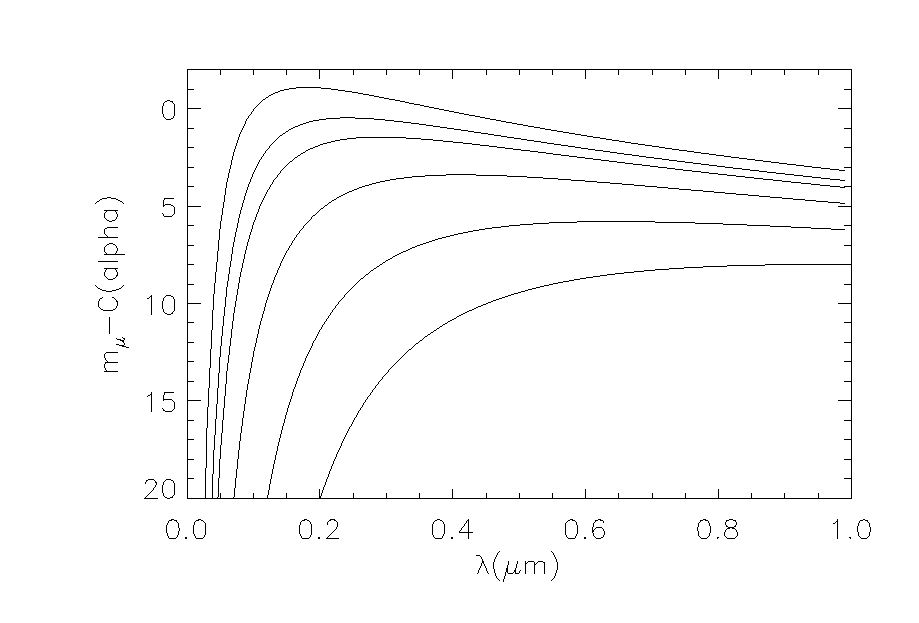
\psfig{file=color_index.eps,width=\textwidth}
	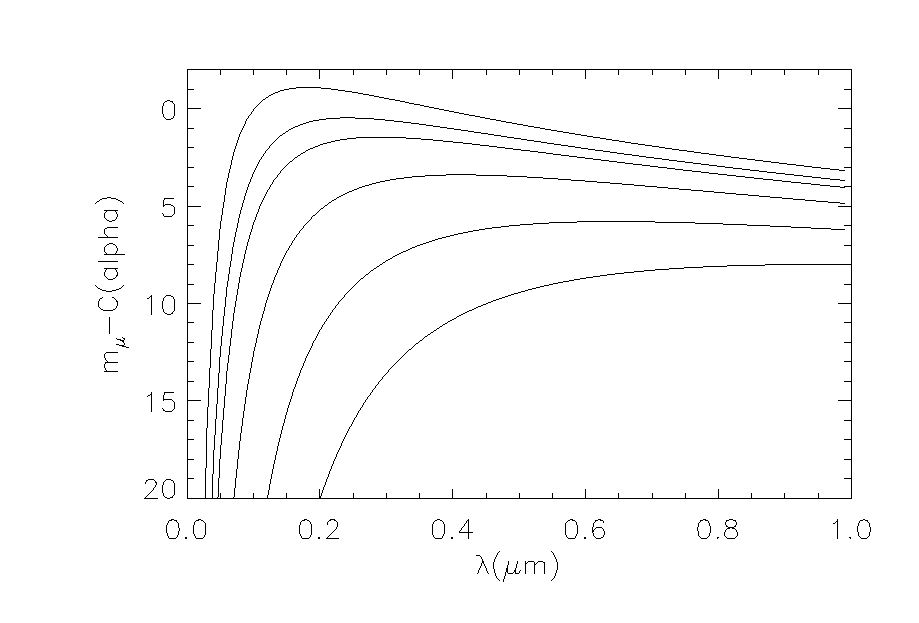
\includegraphics[width=\textwidth]{color_index.eps}
  \caption{Blackbody curves for stars of temperature between $1600$~K
    to $16\,000$~K. $C(alpha)$ is set arbitrarily to $C(alpha)=-15$.}
  \label{fig:color_index}
\end{figure}


\begin{enumerate}
\setcounter{enumi}{\value{count}}
\item Reproduce figure~\ref{fig:color_index} using {\it e.g} {\sc idl}.
\setcounter{count}{\value{enumi}} 
\end{enumerate}

For two (broad) bands centered at $0.4~\mu{\rm m}$ and at $0.8~\mu{\rm
  m}$ is clear that the arithmetical difference between these two
magnitudes for a particular spectrum depends on the average slope of
the spectrum, which in turn depends on the source's temperature. The
convention is to speak of the difference between any two bandpass
magnitudes used to sample the slope of the spectrum as a {\it color
  index}. By convention one computes the index in the sense
\[
{\rm index}=m({\rm shorter}\lambda)-m({\rm longer}\lambda)
\]
The behavior of the color index at the long and short wavelength
extremes of the Planck function are informative. In the Rayleigh-Jeans
region (where $\lambda kT\gg hc$) we have 
\[
m_\lambda=\log{T}+C(\lambda)
\]
so the color index is
\be
(m_{\lambda_1}-m_{\lambda_2})=C(\lambda_1)-C(\lambda_2)=\Delta C
\label{eq:index_rayleigh-jeans}
\ee
which is a constant independent of temperature. At short wavelengths
the {\it Wien approximation} applies and the surface brightness can be
given by 
\[
B(\lambda,T)\approx
\frac{2hc^2}{\lambda^5}\exp\left(-\frac{hc}{\lambda kT}\right).
\]
The color index is then
\be
(m_{\lambda_1}-m_{\lambda_2})=\frac{a}{T}\left(\frac{1}{\lambda_1}-\frac{1}{\lambda_2}\right)+C(\lambda_1)-C(\lambda_2)
\label{eq:index_wien-approx}
\ee
Thus, at very low temperature or short wavelengths the index is a
linear function of $1/T$. 

\begin{enumerate}
\setcounter{enumi}{\value{count}}
\item Show that equations~\ref{eq:index_rayleigh-jeans} and
  \ref{eq:index_wien-approx} are correct.
\setcounter{count}{\value{enumi}} 
\end{enumerate}

\subsection{Line and feature index}
Real objects such as stars will of course have more complex spectra
than blackbodies with features of astrophysical significance such as
absorption and emission lines, bands, and various
discontinuities. Multi-band photometry can measure the strength of
such features. 

Two bands are often sufficient to measure the size of a discontinuity
or the strength of a line. 

The positioning of bands is important. The sensitivity of the index to
the size of the break will diminish if either the bandpass response
includes light from the opposite side of the break. Likewise, if a
band is located too far away from the break, unrelated features can
affect the index. 

An alternative way of characterizing a line is to use two bands ---
one broad, one narrow --- both centered on the line in question. While
the broad band is relatively insensitive, the narrow band is quite
sensitive. The index
\[
{\rm line~index}=m_{\rm narrow}-m_{\rm wide}
\]
tracks the strength of the absorption, in the sense that it becomes
more positive with stronger absorption. One widely used index of this
sort is the $\beta$ index, which measures the strength of the Balmer
beta line of hydrogen, usually useful for luminosity or temperature
classification of stars. 

Finally, note that three bands can be used to measure the {\it
  curvature} or second derivative of a spectrum. Curvature can arise
on relatively short scale because of sharp absorption or emission
lines, or on long scales because of broad or diffuse features such as
molecular bands. A curvature index is defined by the differences
\[
{\rm curvature}=(m_S-m_C)-(m_C-m_L)
\]
where $S$, $C$ and $L$ indicate the short, central, and long
wavelength bands respectively.

\section{Photometric systems}

Photometric systems are defined by at least two specifications:
\begin{enumerate}
\item The wavelength response of each band --- that is, the shape of
  $R_{\rm P}(\lambda)$.
\item Some method for standardizing measurements made in those bands. 
\begin{itemize}
\item Each observer needs to know the value of the constant $C$ that
  will assure agreement of his magnitudes with those of all other
  observers.
\item The different hardware produces some variety in the response
  functions in practice, so a method for standardization must allow
  correction of the inevitable systematic effects due to imperfect matching.
\end{itemize}
\end{enumerate}

The fist specification, $R_{\rm P}(\lambda)$, determines the
{\it instrumental} or {\it natural system}. The first and second
together determine the {\it standard system}. 

Almost all standard systems rely on some network of
constant-brightness standard objects distributed around the sky. It is
important to define a set of standards that include a wide variety of
spectral types.

A {\it closed photometric system} is one in which a small group of
observers carefully controls the instruments and data reduction,
maximizing the internal consistency. Examples include the space borne
HIPPARCHOS data and the Sloane Digital Sky Survey. An {\it open
  photometric system}  is one in which all astronomers are encouraged
to duplicate the defined natural system as best they can, and through
references to a published list of standard stars add to the pool of
observations in the system.

\subsection{Common photometric systems}

\paragraph{Visual and photographic systems} The dark-adapted human eye
determines the band of the {\it visual photometric system}. The
introduction of optical/mechanical visual photometers led to the
establishment of {\it standard sequences} of stars, including
initially the {\it north polar sequence} and later many secondary
sequences: amongst them importantly the 48 Harvard standard regions and the 115 Kapteyn
selected areas.

In the
early twentieth century, astronomers defined two bands based on the
properties of photographic emulsion. The
poor properties of emulsion as a photometric detector, and lack of 
very specific definitions, limited the success of this system. The
{\it international photographic system} is sensitive in the near
ultraviolet--blue region. The response of the {\it international
  photographic photovisual band} roughly corresponds to that of the
visual band ({\it i.e.} the human eye, sensitive to green--yellow). The
IAU in 1922 set the zero point of both magnitudes so that the $6^{\rm
  m}$ magnitude A0 V stars in the north polar sequence would have
(roughly) the same values as on the old Harvard visual system.

\paragraph{The $UBVRI$ system} The most widely used photometric system
prior to the present has been the Johnson-Cousins $UBVRI$ system. This
system was originally based on the RCA 1P21 photomultiplier, a set of
colored glass filters, and a list of magnitudes for a relatively small
number of stars scattered on the celestial sphere. The $V$ band is very
close to the international photovisual band and its zero point was set
so that $V=m{\rm pv}$ for standards in the north polar sequence. The $U$
and $B$ correspond to the short- and long-wavelength bands of the
photographic band, and their zero points are set so that the colors
$U-B$ and $B-V$ are zero for A0 V stars. 

In the period 1960--1965 the system was extended to include bands in
the red $R_J$ and near infrared $I_J$, as well as the longer
wavelength bands $(JHKLMNQ)$ discussed below. Modern work with CCDs
has tended to replace the original $R_J$ and $I_J$ with the $R_C$ and
$I_C$ bands. 

This multi band system was designed with the rough spectral
classification of stars in mind. The $U-B$ index is sensitive to the
Balmeer discontinuity (very obvious in A stars at 370~nm, much reduced
for G stars). The discontinuity  depends on luminosity for hot
stars. The other indices are primarily sensitive to temperature. The
$B-V$ index is more sensitive to metal abundance than $V-R$ or
$R-I$. The $V-I$ index is the most purely temperature sensitive index
in this system. 
\paragraph{The Broadband infrared system: $JHKLMNQ$} This broadband
system might be regarded as an extension of the $UBVRI$ system, it
shares a common zero point so that the colors of an unreddened A0 V
star are zero. Detectors in this region cannot be silicon CCDs but
must be infrared arrays or single-channel infrared devices. 

A large complication for these bands for ground based observations
bandpass definitions can depend critically on atmospheric conditions
(due to water vapor along the line of sight). Different observatories
with identical hardware can experience different infrared window sizes
and shapes if they are at different altitudes. The same observatory
can experience similar bandpass variations due to changing humidity. 

The IAU in 2000 recommended a preferred natural system --- the Mauna
Kea Observatory near-infrared system (MKO).
\paragraph{The intermediate band Str\"omgren system: $uvby\beta$}
Bengt Str\"omgren designed this intermediate-band system in the late
1950s. The system avoids many of the shortcomings of the $UBV$ system
and aims to classify stars according to three characteristics:
temperature, luminosity, and metal abundance. This works well for
stars of spectral types B, A, F, and G provided the photometry is
sufficiently accurate. The four intermediate band colors $uvby$ are
supplemented with a narrow band $\beta$ index which tracks the
strength of the Balmer beta line. This greatly improves the
luminosity classification for hotter stars, and is a good temperature
indicator for cooler stars.

Emission in the $u$ and $v$ bands is depressed by the presence of
metals in a star's atmosphere. Also the $u$ band is depressed by the
Balmer discontinuity. 

\section{From source to telescope}
At least four different effects can alter the photons on their way to
the telescope:
\begin{itemize}
\item wavelength shifts
\item extragalactic absorption
\item Galactic and Solar System absorption
\item atmospheric absorption
\end{itemize}
\subsection{Wavelength shifts}
The photons that leave the source is written $\phi_{\rm
  E}(\lambda_{\rm E}d\lambda_{\rm E}$, where the subscript `E' stands
for ``emitted''. 

Because of the Doppler effect, or because of the expansion of the
Universe, or because of other relativistic effects, the wavelength of
the observed photon will differ from its original value. The new value
is given by
\[
\lambda_o=(1+z)\lambda_{\rm E}
\]
where $z$ is the redshift parameter $z={(\lambda_o-\lambda_{\rm
  E})/\lambda_{\rm E}}$ of the source. The number of photons is
conserved in these processes so 
\[
\phi(\lambda)d\lambda=\phi_{\rm E}(\lambda_{\rm E}d\lambda_{\rm E}
\]
Thus, the observed and emitted monochromatic photon flux are related by 
\[
\phi(\lambda)=\frac{1}{1+z}\phi_{\rm E}\left(\frac{\lambda}{1+z}\right)=f_\lambda\frac{\lambda}{hc}
\]
and the monochromatic flux density is then
\[
f_{\rm E}(\lambda_{\rm E})=f_{\rm
  E}\left(\frac{\lambda}{1+z}\right)=\frac{hc\phi_{\rm E}(\lambda_{\rm
    E})}{\lambda_{\rm E}}=(1+z)^2f_\lambda
\]
Note that the monochromatic flux density is {\it not} conserved.

An observer who uses a bandpass with photon response $R(\lambda)$ will
measure the magnitude
\bua
m_{\rm R}&=&-2.5\log
{ \int R(\lambda)\frac{\phi(\lambda)}{\lambda}d\lambda}+C_{\rm R} \\
C_{\rm R}&=&-2.5\log{\int   R(\lambda\frac{g_\lambda}{hc}d\lambda}
\eua
where $g_\lambda$ is the spectrum of a photometric standard magnitude
zero. We need to find how $m_{\rm R}$ relates to a magnitude measured
for these same photons before their wavelength shift. Call the
unshifted band the photons began their journey in $Q$, different from $R$.

\bua
m_{\rm Q}&=&-2.5\log{\int
  Q(\lambda)\frac{\phi_{\rm E}(\lambda)}{\lambda}d\lambda}+C_{\rm Q} \\
                &=&-2.5\log\left[{(1+z)\int
                    Q(\lambda)\frac{\phi(\lambda(1+z))}{\lambda}d\lambda}\right]+C_{\rm
                  Q} \\
C_{\rm Q}&=&-2.5\log{\int   Q(\lambda\frac{g_\lambda}{hc}d\lambda}
\eua
We must consider the difference
\[
m_{\rm R}-m_{\rm Q}=2.5\log(1+z)
+C_{\rm R}-C_{\rm Q}+2.5\log\left[
  \frac{\int  Q(\lambda)\frac{\phi(\lambda(1+z))}{\lambda}d\lambda}{\int R(\lambda)\frac{\phi(\lambda)}{\lambda}d\lambda}\right]
\]
For objects in our galaxy, $z$ is small, and one can use
$R(\lambda)=Q(\lambda)$, $C_{\rm R}=C_{\rm Q}$, in which case the
first three terms add up to zero. The last term describes the effect
of photons shifting into and out of the band. In the case of narrow
bands near sharp spectral features, even small Doppler shifts can
produce large differences between $\phi((1+z)\lambda)$ and
$\phi(\lambda)$. 

For distant objects $z$ becomes large because of the expansion of the
Universe. Given knowledge of $\phi(\lambda)$ and $z$ it is possible to
use an observed bandpass magnitude to compute the magnitude that
would be observed if the source had a redshift $z=0$. Hubble called
this kind of correction the {\it K correction}. 
%
\subsection{Absorption outside the atmosphere}
Interstellar gas and dust absorb and scatter light. It is common to
refer to both processes as ``absorption''. Absorption not only reduces
the number of photons arriving at the telescope, {\it extinction}, but
also alters the shape of the spectrum.

Diffuse gas absorbs photons to produce {\it interstellar absorption
  lines and bands}. In the optical sodium D is usually the strongest
interstellar line, in the UV the Lyman-alpha line is usually
strongest. At short wavelengths gas will also produce continuous
absorption and absorption edges due to ionization {\it e.g.} at
$91.2$~nm due to the Lyman continuum. Absorption by dust will
generally alter the overall shape of the spectrum. In the region
$0.22-5.0~\mu{\rm m}$, dust scatters short wavelength photons more
than long wavelength photons, so the resulting change in shape of the
spectrum is called {\it interstellar reddening}. 

Now define $S_{\rm
  ism}(\lambda)$ as the fraction of photons of wavelength $\lambda$
that are transmitted by the interstellar medium within our galaxy and
$S_{\rm exg}(\lambda)$ as the fraction of photons arriving at
$\lambda$ that are transmitted by the interstellar medium outside our
galaxy. Note that because of cosmological redshift, absorption
described by $S_{\rm exg}(\lambda)$ involve photons that had
wavelength ${\lambda/(1+z')}$ when they were absorbed by material with
  redshift parameter $z'$. (This produces the phenomenon of the {\it
    Lyman-alpha forest} in the spectra of distant objects: multiple
  absorption lines due to Ly $\alpha$ at multiple red-shifts.) The
  photon flux that reaches the top of the Earth's atmosphere is 
\[
\phi(\lambda)=S_{\rm ism}(\lambda) S_{\rm
  exg}(\lambda)\phi_0(\lambda)=S_{\rm ism}(\lambda) S_{\rm
  exg}(\lambda)\frac{1}{1+z}\phi_{\rm E}((1+z)\lambda)=f_\lambda\frac{\lambda}{hc}
\]
where $\phi(\lambda)$ is the photon flux outside the atmosphere and
$\phi_0(\lambda)$ is the photon flux outside the atmosphere corrected
for interstellar absorption. 
%
\subsection{Absorption by the atmosphere}
Extinction in the Earth's atmosphere is a strong function of
wavelength. At sea level, three opaque regions define two transmitting
windows. Rayleigh scattering and absorption by atoms and molecules
cause a complete loss of transparency at all wavelengths shorter than
about 300~nm. This sets the short end of the {\it optical infrared
  window}. The second opaque region, from absorption in molecular
bands --- primarily due to H$_2$O and CO$_2$ --- begins at roughly
$0.94~\mu{\rm m}$, has a few breaks in the infrared and mid infrared,
and extends from 30~mm to the start of the {\it microwave radio
  window} at around 0.6~cm. The radio window ends at around 20~m
because of ionospheric absorption and reflection.

Qualitatively we can set up an atmospheric transmission function
$S_{\rm atm}(\lambda,t,e,a)$ as the fraction of photons of wavelength
$\lambda$ that are transmitted by the Earth's atmosphere at time $t$,
elevation angle $e$ and azimuth $a$. The photon flux that reaches the
telescope is then

\[
\phi_{\rm A}(\lambda)=S_{\rm atm}(\lambda,t,e,a)S_{\rm ism}(\lambda) S_{\rm
  exg}(\lambda)\frac{1}{1+z}\phi_{\rm E}((1+z)\lambda)=f^{\rm A}_\lambda\frac{\lambda}{hc}
\]
and the rate at which energy gets detected in an infinitesimal band is 
\[
dE_{\rm sig}=aT'_{\rm P}(\lambda)f^{\rm A}_\lambda d\lambda=aT'_{\rm
  P}(\lambda)\frac{\phi_{\rm A}(\lambda)}{\lambda}d\lambda
\]
Where $a$ here is the effective collecting area of the telescope, and
$T'_{\rm P}(\lambda)$ is a function of the overall wavelength
dependent efficiency of the instrument. Integrating this equation
gives us the {\it instrumental magnitude}
\bua
m^{\rm A}_{\rm P}&=&
-2.5\log\int T'_{\rm
  P}S_{atm}(\lambda)\frac{\phi(\lambda)}{\lambda}d\lambda+C'_{\rm P}
\\
&=&m_{\rm P}^{\rm O}+A_{\rm atm}+A_{\rm ism}+A_{\rm exg}+C^{\rm
  z}_{\rm P} \\
&=&m_{\rm P}+A_{\rm atm}
\eua
Here the $A$ parameters represent the atmospheric, Galactic, and
extragalactic absorption, in magnitudes; $C_{\rm P}^z$ is the
correction for wavelength shift; and $C'_{\rm P}$ is the constant that
sets the zero point of the instrumental magnitude scale. The quantity
$m_{\rm P}$, the {\it instrumental magnitude outside the atmosphere},
depends on the telescope and photometer but is independent of the
atmosphere. The quantity $m_{\rm P}^{\rm O}$ is the instrumental
magnitude in the emitted frame corrected for all absorption
effects. $m_{\rm P}$ can be written as
\[
m_{\rm P}=-2.5\log\int T_{\rm
  P}\frac{\phi(\lambda)}{\lambda}d\lambda+C_{\rm P}
\]
where $T_{\rm P}(\lambda)$ and $C_{\rm P}$ characterize the
instrumental system located outside the atmosphere.
%\end{document}
